% Author: Animesh Garg
% Date: June 23, 2013

\section{INTRODUCTION}
\label{sec:introduction}
% Motivate the problem

Every year, \todo{X} cases of cancer are treated with Radiation therapy 
in United States.
External Radiation Therapy, along with its variations, is a common form
of radiotherapy treatment. With external radiation therapy, radiation is usually 
administered as a complex combination radiation beams directed at the tumor. 
Advanced techniques of dose 
calculation and treatment delivery are employed to permit design of treatment 
fields to maximize the differential in dose delivered to tumors and healthy 
tissue.

Accuracy and precision in patient positioning is essential for success of 
external radiation delivery systems. Since radiation therapy is delivered over 
multiple sessions, repeatability of a patient positioning system is important 
to maintain registration between the patient and radiation delivery equipment.

Presently, a variety of patient positioning  systems are employed in clinical 
procedures. However, most if not all of these systems are one-size-fits-all. 
This leads to problems in maintaining conformance between
simulated and physically delivered radiation dose distributions over multiple 
sessions. Furthermore, these patient positioning systems are inconvenient 
for the patients often requiring local anesthesia to relieve pain.

%Give example of the problem
For instance, stereotactic radiotherapy (SRT) is used primarily for treating 
tumors in the brain. The procedure has sub-millimeter accuracy, but assumes 
exact patient to machine registration. Commercially available head positioning 
solutions for SRT usually require the patient's head to be placed in a cubical 
frame with multiple pegs securing the head in its place. One example of such
a system is illustrated in figure~\ref{fig:leskellFrame}. These pegs are 
uncomfortable and the the frame only allows the head to be placed in a 
small set of orientations.

Additionally, the ability to easily position the head in any orientation simplifies
planning for radiation dose in external radiation therapy. For e.g., if a patient 
is immobilized in a non-supine position, reaching tumor might become easier 
due to decreased hindrance from healthy tissue. 


%state our solution
The key insight in building a principled solution for immobilization is 
customization to patient anatomy. We propose a solution which leverages 
redundant point contacts  and uses surface contacts. 
This higher degree of customization is also facilitated by
recent advances in additive manufacturing and 3D printing.

After a 3D reconstruction of the patient anatomy using a CT (or MRI) scan,
we use redundant contact points and surface contacts to the set of minimal 
grasp points required for immobilization. This reduces maximum force at any
contact point. The benefit of inclusion of additional contact points is a 
submodular function, which allows us to find the optimal set in reasonable time. 

%list claims and their significance. (Use forward referencing instead of explicit roadmap of the paper. )
This study builds upon the previous work from Schulman et al 
\cite{schulman2011grasping}. In this paper,
\begin{itemize}
\item We describe an algorithm which minimizes maximum contact force and 
immobilizes the subject.
\item We evaluate the performance of algorithm on multiple instances of \todo{X} 
body parts.
\item We create a patient specific head positioning system using 3D printing.

\end{itemize}

\begin{figure}[t!]
  \begin{center}
    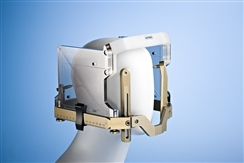
\includegraphics[width=0.8\linewidth]{images/leskellFrame}
  \end{center}
  \vspace{-10pt}
\caption{ The figure shows a Leskell Coordinate Frame G used for Stereotactic Radiosurgery.
As illustrated in the picture, the patient head is placed in a frame and secured in place with 
use of multiple pins}
  \vspace*{-15pt}
  \label{fig:leskellFrame}
\end{figure}
